\chapter{Resumen y Conclusiones}
\label{chap:conclusions}
\thispagestyle{empty}
%Write Conclusions, discussions, etc. here
%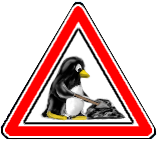
\includegraphics[width=0.1\linewidth]{./Figures/tux-development}

En el capítulo \ref{chap:bow-shocks} mencionamos escenarios astrofísicos donde se forman choques de proa para resaltar las diferentes situaciones donde se puede aplicar el trabajo desarrollado en esta tesis, entre las que hemos destacado las siguientes:

\begin{itemize}
\item Proplyds.
\item Objetos LL
\item Estrellas errantes
\item Estrellas AGB y supergigantes rojas
\end{itemize}

En el capítulo \ref{chap:ONC} mencionamos el modelo aceptado para los proplyds, que consiste en que el disco protoplanetario de una estrella tipo T Tauri embebida dentro de una región \Ion{H}{II} está siendo fotoevaporado e ionizado por la radiación ultravioleta de la estrella masiva central. Se forma un frente de ionización con forma aproximadamente hemisférica entre la estrella T Tauri y la estrella masiva y una cola que apunta en dirección opuesta que se forma cuando el disco protoplanetario es fotoevaporado e ionizado por la radiación difusa.

En el caso particular de ON, en muchos de los proplyds también se observan choques de proa, que son resultado de la interacción del flujo fotoevaporado del proplyd con el viento estelar de \thC{}. Trabajos previos \citep{Robberto:2005}, intentaron comparar la forma de los choques de proa más cercanos a \thC{} con el modelo de capa delgada de \citet{Canto:1996} midiendo en observaciones en infrarrojo a \SI{10}{\mu.m} los radios proyectados $R_0$ y $R_{90}$ normalizados con la distancia proyectada $D$ a \thC{}. Sin embargo, no todas las mediciones concuerdan con las predicciones del modelo de capa delgada \ref{fig:Robberto}.

En el capítulo \ref{chap:Modelo-generico} describimos los conceptos más importantes para describir la forma de un choque de proa cilíndricamente simétrico producto de la interacción de dos vientos en estado estacionario bajo tres escenarios (figuras \ref{fig:crw-esquema} y \ref{fig:isotropic-aniso}):

\begin{itemize}
\item Un viento interior esférico, isotrópico, supersónico y no acelerado interactúa con un viento plano--paralelo con velocidad constante e hipersónica y densidad constante. Al choque resultante se le conoce como \textit{wilkinoide}.
  \item Un viento interior supersónico y no acelerado que puede ser a) esférico e isotrópico o b) hemisférico y con densidad que varía con el ángulo polar como una ley de potencias de $\cos\theta$ con índice de potencias $k$ que interactúa con un viento exterior esférico, isotrópico, hipersónico y no acelerado. A los choques resultantes se les conoce como a) \textit{cantoides} y b) \textit{ancantoides}, siendo estos últimos una extensión al trabajo previamente publicado de \citet{Canto:1996}, con el fin de lograr que las mediciones faltantes ajustaran con las nuevas predicciones teóricas de este tipo de choques.
\end{itemize}

La forma de un choque de proa se puede caracterizar con una serie de parámetros que pueden obtenerse de manera observacional para choques de proa en imágenes en cualquier longitud de onda siempre y cuando la imagen esté resuelta, que son al radio en el ápex, la planitud y la alatud (figura \ref{fig:char-radii}). 

Desarrollamos de manera independiente (ver por ejemplo \citet{Wilkin-thesis}) un método para encontrar la forma proyectada de un choque de proa cilíndricamente simétrico en un marco de referencia que está rotado por un ángulo $i$ respecto al plano del cielo, suponiendo que sea visible su \textit{línea tangente} por abrillantamiento al limbo. Aplicamos este método primero a superficies cuádricas, tales como hiperboloides, esferoides, paraboloides y elipsoides, donde la línea tangente es una sección cónica. Encontramos la dependencia con inclinación de la planitud y la alatud proyectada, en forma de funciones explícitas, así como curvas dependientes de la inclinación en el plano $\Pi'-\Lambda'$ y encontramos que dependiendo del tipo de superficie, cuantificada por el parámetro $\Q{}$, éstas se mueven en tres diferentes regiones (figura \ref{fig:Pip-Lambdap-diagnostic}a): la región superior (hacia alatudes altas), donde se encuentran los hiperboloides. Una región intermedia y angosta donde se encuentran los elipsoides prolatos, y la región inferior donde se encuentran los elipsoides oblatos. Los paraboloides se encuentran exclusivamente en la interfaz entre la región de los hiperboloides y los elipsoides prolatos. Y los esferoides se encuentran en la interfaz entre los elipsoides prolatos y oblatos. También se encontró que conforme $i\to 90^\circ$, la planitud y alatud aparentes convergen a $\Pi'=\Lambda'=1$ para los elipsoides y esferoides, y los paraboloides convergen a $\Pi'=\Lambda'=2$. para los hiperboloides la planitud y alatud aparentes divergen cuando la inclinación tiende a un valor crítico donde deja de existir la línea tangente.

En el capítulo \ref{chap:hipersonica} describimos a detalle el modelo de capa delgada de \CRW{} para los tres escenarios de interacción de vientos ya descritos. Calculamos la planitud, la alatud y el ángulo asintótico $\theta_\infty$ de los choques resultantes en función de los parámetros del modelo que son el cociente de la tasa de momentos $\beta$ y el parámetro de anisotropía $k$ en el caso de los choques ancantoides. A diferenia del caso de las cuádricas de revolución, aquí no existen funciones explícitas para describir la forma del choque resultante. A partir de la planitud y la alatud se puede aproximar la forma de la cabeza y de las alas lejanas del choque a una cuádrica de revolución. La forma de las alas lejanas siempre ajusta a un hiperboloide, mientras que para la cabeza ajusta mejor a un esferoide prolato cuando el cociente de las tasas de momentos $\beta$ es pequeño y conforme este parámetro se incrementa, la forma de la cabeza pasa a ser hiperbólica (figura \ref{fig:thq-beta}).

Siguiendo el método del capítulo anterior, encontramos la forma proyectada de los choques en el modelo de capa delgada y calculamos la planitud y alatud aparentes en función de la inclinación. Excepto para los choques wilkinoides, la planitud y la alatud aparente incrementan con inclinación. La planitud aparente de los choques ancantoides presenta una discontinuidad en inclinaciones tales que la línea tangente pasa por $\theta=90^\circ$ donde la segunda derivada de $R(\theta)$ tiene una discontinuidad debido a que en ese punto termina el viento interior.

En este modelo las curvas dependientes de la inclinación en el diagrama planitud-alatud son más complicadas que en el caso de las cuádricas de revolución, y no se encuentran confinadas a una sola región. De manera general la forma aparente del choque es más parecida a un esferoide prolato a inclinaciones bajas y a un hiperboloide a inclinaciones altas. Esto debido a que la línea tangente se va recorriendo hacia las alas lejanas conforme la inclinación aumenta, donde la forma del choque se aproxima más a un hiperboloide.

En el capítulo \ref{chap:proplyds} hicimos mediciones de la planitud, el radio aparente $R'_0$ en el ápex y la distancia proyectada $D'$ de los choques de proa asociados a los proplyds clásicos LV2--LV5 y otros proplyds cuya distancia proyectada es mayor: 168-338, 169-338, 177-341 (HST1) y 180-331 con imágenes del HST en el filtro F502N tomadas con el instrumento WFPC2. Debido a que el brillo superficial es menor en dirección a las alas, la alatud proyectada no es medible. La forma los choques de proa fue medida con marcas puntuales a lo largo de cada choque utilizando las herramientas del programa DS9 para imágenes astronómicas, así como para la posición de cada proplyd y la de \thC{}, y extrayendo las coordenadas de cada marca. El radio de curvatura fue medido haciendo un ajuste de mínimos cuadrados a un círculo de las marcas que trazan la posición de los choques y $R'_0$ fue medido como la distancia entre el proplyd y el ajuste en la línea que conecta la posición del proplyd con \thC{}. Se repitió el proceso con 10 sub-muestras donde en cada una de ellas se removió la tercera parte de las marcas originales de manera aleatoria. Las desviaciones en las mediciones de la planitud y $R'_0$ de cada sub-muestra respecto a la medición original juegan el papel de las incertidumbres. Se compararon estas mediciones con las predicciones teóricas del modelo de capa delgada en diagramas planitud vs $R'_0/D'$ asumiendo un valor fijo para el parámetro de anisotropía $k$, y por medio de inspección visual se estimaron posibles valores para la inclinación y el cociente de tasas de momentos $\beta$ para cada proplyd. A partir de estas determinaciones se estimó la distancia intrínseca $D$ y el radio intrínseco en el ápex $R_0$. Por último, utilizando mediciones del radio del frente de ionización de \citet{Garcia-Arredondo:2001}, evaluamos las condiciones de equilibrio de ionización y de presiones, mostradas en la figura \ref{fig:wind-fits}, bajo dos suposiciones para la densidad del viento interior: a) que la condición de equilibrio de presiones no se cumple ``de facto'' por lo que utilizamos la densidad del frente de ionización reportada en \citet{Garcia-Arredondo:2001} y b) La condición de equilibrio de presiones sí se cumple ``de facto'' y la densidad pre-choque del viento interior es calculada a partir de la ecuación \ref{eq:b-density}. Para la tasa de momento del viento exterior utilizamos los parámetros de \citet{GAH:2002} y el modelo frío de \citet{Gagne:2005}, donde ambos cumplen con la condición $\dot{M}_{-7}/v_{3} \sim 2$. Hasta este punto no queda claro cuál de los modelos para el viento exterior predice un mejor ajuste a la condición de equilibrio de presiones en cada choque de proa.

\section{Trabajo a Futuro}

El contenido del capítulo \ref{chap:proplyds} será incluído en un artículo para ser enviado posteriormente a una revista para su publicación. Con el fin de poder concluir con las determinaciones de la densidad del viento interior y evaluar de manera más eficaz las condiciones de equilibrio de ionización y presiones ram, hace falta establecer un método más eficiente para estimar la inclinación al comparar las mediciones con el modelo de capa delgada en función de los parámetros $(\beta, k)$, y a su vez establecer un método para cuantificar el grado en que las estimaciones de la inclinación se aproximan a las condiciones de equilibrio de ionización y presión ram. A su vez es necesario explorar otros modelos donde se formen choques de proa.

En artículos aún en preparación, se analiza diferentes escenarios donde además de la interacción viento--viento consideramos además escenarios donde la radiación de la estrella y el acoplamiento entre gas y polvo del ambiente juegan un papel importante (ver apéndice \ref{app:future-work}). Finalmente, en la \S 6 de \citet{Tarango-Yong:2018a} se hizo un análisis de las formas de los choques de proa resultantes de simulaciones hidrodinámicas y magnetohidrodinámicas de \citet{Meyer:2017} que incluyen las predicciones de la forma aparente de la discontinuidad de contacto en el diagrama $\Pi'$--$\Lambda'$ en forma de curvas dependientes de la inclinación, el radio aparente en el ápex $R'_0$ en función de la inclinación, etc. con el fin de comparar estos modelos con observaciones de las formas de los arcos por estrellas errantes. 
%Hemos desarrollado un método para caracterizar la forma geométrica de choques de proa comparando dos parámetros adimensionales: la \textit{planitud} $\Pi$ del ápex del choque, y la \textit{alatud} $\Lambda$, o abertura de las alas. Ambos pueden ser medidos como los cocientes de longitudes que pueden ser medidas fácilmente. Desarrollamos un método (\S \ref{sec:projection}) para encontrar la forma aparente $(\Pi', \Lambda')$ de un choque abrillantado al limbo que es idealizado como cilíndricamente simétrico, en función del ángulo de inclinación $i$. Aplicamos este resultado a las cuádricas de revolución (capítulo \ref{chap:Modelo-generico}) y a la forma de los choques resultantes del modelo de capa delgada de interacción de dos vientos de \CRW{}, que están clasificados como wilkinoides, cantoides y ancantoides (capítulo \ref{chap:hipersonica}), y a observaciones en óptico de los choques de proa observados en la vecindad del Trapecio, en el centro de ONC (capítulo \ref{chap:proplyds}).

%Aunque ya se han hecho análisis a las formas geométricas de los choques de proa (\citet{Robberto:2005}, ver figura \ref{fig:Robberto}), no se había utilizado antes el parámetro de la \textit{planitud} que siempre puede ser medido, a diferencia de la alatud, como ya ejemplificamos en el capítulo \ref{chap:proplyds}.

%A pesar de que mucho del contenido de la \S \ref{sec:projection} ya había sido reportado en \citet{Wilkin-thesis} (apéndice B), las ecuaciones mostradas en esta sección fueron desarrolladas de manera independiente.

%Se introdujo el diagrama $\Pi-\Lambda$ como una manera de caracterizar la forma de choques de proa. Las cuádricas de revolución sirven para caracterizar distintas regiones de este diagrama, y sirven como primera aproximación a la forma geométrica de otras superficies más complicadas.

%En el modelo de capa delgada de \CRW{} (capítulo \ref{chap:hipersonica}), los escenarios que forman los choques cantoides y wilkinoides forman parte del trabajo de \CRW{}, siendo los choques ancantoides una extensión a este modelo. Por otro lado, el término \textit{wilkinoide} fue acuñado inicialmente por \citet{Cox:2012}, y a partir de ese nombre se acuñaron los términos \textit{cantoide} y \textit{ancantoide}.

%Las mediciones del radio aparente en el ápex de los choques de proa cercanos al Trapecio en ONC concuerdan con las mediciones realizadas por \citet{Robberto:2005} (excepto por LV3). Además, comparando la forma aparente en un diagrama $(\Pi'-\frac{R'_0}{D'})$ de los choques con la forma aprente que predicen los modelos de capa delgada de \CRW{}. Encontramos los parámetros $(\beta, k, i)$ en los que coinciden los modelos con las observaciones. A partir de estos parámetros y utilizando las mediciones del radio del frente de ionización de cada proplyd medidos en \citet{HA:1998}, la tasa de pérdida de masa y la velocidad terminal de \thC{} de \citet{Gagne:2005}, dos modelos para estimar la densidad máxima del Frente de Ionización de los proplyds y números de Mach del flujo evaporado en el rango $[2, 3]$, encontramos que la dependencia con el número de Mach no es muy fuerte, que en el modelo A para estimar la densidad del IF del proplyd no existe correlación entre la presión encontrada con la distancia a \thC{}, mientras que en el modelo B sí existe, y dado el ajuste entre este modelo y las mediciones de la presión, el modelo B sería preferible. En trabajos posteriores se piensa analizar con el diagrama $\Pi-\Lambda$ a las clases de choque de proa mencionados en las \S \ref{sec:Luis-LL}, \ref{sec:runaway} y \ref{sec:AGBs}.
